\documentclass{article}
\usepackage{lmodern, amssymb,amsmath, graphicx, hyperref}
% === bibliography package ===
\usepackage{natbib}
% \usepackage[colorinlistoftodos, prependcaption]{todonotes} % to use \todo 
\usepackage[margin=1in]{geometry}
\usepackage{csquotes}
\usepackage{setspace}
\hypersetup{
    colorlinks=true,
    linkcolor=blue,
    filecolor=magenta,      
    urlcolor=cyan,
    citecolor = black
}
\urlstyle{same}  % don't use monospace font for urls

  \title{Using Constituency Service to Understand Inequality, Money in Politics and Legislative Behavior}
    \author{Devin Judge-Lord\thanks{Ph.D. Candidate, University of Wisconsin-Madison}\and Justin Grimmer\thanks{Professor, Stanford University} \and Eleanor Neff Powell\thanks{Booth Fowler Associate Professor, University of Wisconsin-Madison}}
    \date{\today}
    
\graphicspath{{gh-pages/Figs/}}


\begin{document}

\maketitle
% \tableofcontents

% \bigskip
% \href{https://judgelord.github.io/correspondence/gh-pages/summary.html}{Project Summary} | 
% \href{https://docs.google.com/document/d/1fJxjXjAyRL9vX-16fSsH29anXZc-W74GMf_7BSgWkws/edit}{Codebook} |
% \bigskip

\begin{abstract}
\noindent Representation in Congress is based, in part, on legislators' ability to assist their constituents with the federal bureaucracy.  Constituency service is central to definitions of representation as well as empirical explanations for phenomena such a the incumbency advantage. And yet, too little is known about when and how elected officials contact the bureaucracy on behalf of their constituents. We assemble a massive new database of over 150,000 Congressional requests to agencies between 2007 and 2017 obtained through over 250 FOIA requests, approaching a census of all contacts with the bureaucracy. We examine when legislators contact agencies, which legislators contact those agencies, and the purpose of the contact.  Our work provides new insights into who provides constituency service, why they provide that service, and the consequences of the agency requests for how governments make decisions. % Not only do representative vary significantly in their productivity, the top advocates for individual constituents are also the top advocates for policy change, making contact with the bureaucracy an important dimension of representation.
\end{abstract}

\newpage
\doublespacing
\section{Introduction}
One of the oldest traditions of legislative representation in American politics is that of constituency service---the ways in which legislators help to channel and articulate individual constituent's requests to the government.  This tradition dates back to the first congresses when constituents sought assistance with Revolutionary War pensions \citep{Eckman2017}. Today constituents seek assistance with a wide range of topics from Social Security, Disability, and Veterans Benefits to Citizenship Applications to complaints about pollution and employment discrimination. Members also serve constituents by advocating on behalf of state or local governments or nonprofits who apply for federal grants, permits, or disaster recovery funds. % \todo{include other examples of constituency service} \citep{Eckman2017}  
Advocating on behalf of their constituents to federal agencies is an important facet of modern legislators' jobs, and its growth has been used to explain the presence of the incumbency advantage \citep{King1991}.  

Yet despite the centrality of constituency service in theories of congressional representation, constituency service remains one of the most opaque and least understood congressional activities. Indeed, we are not the first to observe the relative lack of empirical attention to constituency service in the literature.  Over thirty years ago \citet*{CainFerejohnFiorina1987} began their seminal book \emph{The Personal Vote: Constituency Service and Electoral Independence} with that same observation, and much of what we know empirically today about constituency service is due to their surveys of legislators, legislative staff, and constituents.  While this evidence is second best, it has been used to help explain who provides constituency service, how a legislator's demographics and institutional position affect the kind of service they provide, and the extent to which legislators provide special favors for political donors or other moneyed interests.  

Given the importance of these classic empirical questions about constituency service, we employ a new data set to assess constituency service and its consequences.  In this project, we employ the most comprehensive dataset of constituent service requests to date.  Using a large set of Freedom of Information Act (FOIA) requests we have been able to assemble a large data set of nearly every instance of when legislators contact government agencies on behalf of their constituents.  Other scholars working with similar, though less extensive, data have shown that the data on congressional correspondence has yielded important findings regarding the policy strategies of cross-pressured legislators \citep{Ritchie2017}, distributive politics \citep{MillsKalafHuges2015}, descriptive representation \citep{LowandeRitchieLauterbach2018}, and the role of ideology in congressional oversight \citep{Lowande2018JOP}.  

In this project, we build on this important work to tackle long-standing questions about who provides constituency service, why they provide that service, and how legislators advocacy for constituents can perpetuate inequality in access to policy influence.  To make these contributions we introduce a new data set of Congressional correspondence obtained through over 200 Freedom Of Information Act (FOIA) requests.  This comprehensive dataset enables us to make inferences about how legislators generally allocate their time, while more prior more narrow data sets have forced scholars to restrict attention to the legislator-agency dyad.  In this proposal, we provide a summary of the data that we have already collected and show that even the descriptive facts in the data provide insights into how legislators allocate their time.  In addition to collecting the data, we use the information provided by federal agencies to classify why the constituency service request was made.  This enables us to home in on particular kinds of service requests. 

We will make available our comprehensive data set, enabling other scholars to learn from the extensive data that we have collected.  In order to allay concerns about the comprehensiveness of our data, we provide several validations of the validity and will use grant funding to further clarify what the data can and cannot explain. Our new datasets will facilitate a wide array of research on how legislator behavior and government decisionmaking.    

In this grant proposal, we provide examples of how the data can be used to both study legislator behavior and how government decisions are made.  We first establish some previously unknown but important descriptive facts about who makes requests to federal agencies. There are a few members who use this tactic much more often than their colleagues.  And these differences cannot be explained away by conditioning on institutional power, experience, staffing resources, or national prestige. Furthermore, those who use this tactic use it broadly across issue areas and parts of the government.  Members of Congress who write often to one agency are more likely to write regularly to other agencies as well.  In general, the legislators who engage the bureaucracy do so broadly, across many agencies and advocate both for general policy and for individual constituents.  Using this data, we plan to develop a basic measurement model to more systematically describe the strategies that legislators deploy when contacting federal agencies. 

Our comprehensive data set and panel research designs provide us with useful causal leverage on what effects legislators' propensity to contact some federal agencies.  It also gives us leverage on a variety of causal questions about how institutional position and rules affect the rate of contact of federal agencies and to characterize the ability of moneyed interests to receive extra attention.  We show that after legislators gain more institutional prestige---becoming a committee chair, gaining a set on a prestige committee, or moving into party leadership---they contact \emph{more} federal agencies.  Using a difference-in-differences research design, we show that these differences are not merely attributable to high-capability legislators being selected for leadership positions.  that said, we do show that legislators selected for promotions tend to contact more than other legislators before the promotion.  

Using this basic research design, we are also able to assess how legislators' constituent service requests affect government decision making.  A recent innovation in Congress has been to eliminate lawmakers ability to earmark funds for their district: lawmakers are no longer able to explicitly allocate funds for pet projects in their districts.  Of course, a reasonable concern might be that legislators can use constituent service requests instead of earmarking to secure funds for their district.  We can contact two types of studies to assess whether it is plausible that letters to agencies have replaced earmarks in federal funding decisions.  As we explain in more detail below, we will examine how agency requesting patterns shift after an earmark ban. If more requests are made to agencies that allocate money, we have superficial evidence of an attempt to influence decision making.  A second research design will enable us to better understand the effect of constituent service requests on government decisions.  Specifically, we will link requests in support of grant application with public records on whether specific grants were allocated.  Using this design we can assess the relationship between letters written in support of an application and the agency's funding decisions.  


Together, our results provide new and important insights into how constituency service is provided in American politics and its consequences for how government decisions are made.  Using our comprehensive data set, we are able to provide new insights into who provides representation to constituents and what groups are advantaged.  And by assessing the effect on government decision making, we are able to assess if moneyed interests---such as businesses or local governments with access to lobbyists---are advantaged in the allocation process. 

\subsection{What is constituency service?}

One of the earliest and most comprehensive academic descriptions of constituency service comes from Richard Fenno in his classic book \emph{Home Style: House Members in Their Districts}. As Fenno describes:

\begin{displayquote}
Many activities can be incorporated under the rubric of `district service,' or `constituent service,' but the core activity is providing help to individuals, groups, and localities in coping with the federal government.  Individuals need someone to intercede with the bureaucracies handling their veterans' benefits, social security checks, military status, civil service pension, immigration proceedings, and the like.  Private groups and local governments need assistance in pursuing federal funds, for water and sewer projects, highways, dams, buildings, planning, research and development, small business loans, and so forth \citep[pg. 101]{Fenno1978}.
\end{displayquote}

While the definition that Fenno presents is broad, the central element is clear -- assisting constituents (individuals or groups) in interacting with government agencies.  Fenno's description is consistent with how \citet[pg. 2]{CainFerejohnFiorina1987} characterize constituency service as acting as an ``ombudsman'' for constituents vis-a-vis the administrative state.  These scholarly definitions of constituent service from \citep{Fenno1978} and \citet{CainFerejohnFiorina1987} are consistent with how legislators understand the concept today, and according to a recent Congressional Research Service Report constituency service ``is commonly considered a representational responsibility'' \citep{Eckman2017}.  It is worth noting that this definition of constituency service is an expansive one that encompasses both individual casework activity (e.g. requests for assistance with a social security check) and district- or group-level advocacy. It does not hinge on a precise definition of which individuals and groups count as constituents. Representatives may advocate for groups that are organized and intense demanders of government benefits or protections (e.g. support for a local union facing a factory closing) or merely linked by a common fate (e.g. general support for hurricane recovery aid in the district). The key distinction in this notion of constituent service is that it is an act of service to a particular individual or group at a particular time, rather than a broad or enduring policy that may apply to many groups over time. 

% note: our coding scheme captures casework + district/group-level advocacy--e.g. general support for hurricane recovery or refugees. 

% \subsection{Why do legislators perform constituency service?}

% To understand why legislators engage in constituency service, we begin with the broader question of what motivates Members of Congress?  The classic answers come from \citet{Mayhew1974} and \citet{Fenno1973}. In \emph{Congress: The Electoral Connection}, Mayhew argues that re-election is the primary (or at least the proximate) motivation because it is a necessary step to achieve other goals (such as policy or power within Washington). Constituency service activity has traditionally been viewed as a way to improve one's re-election prospects by assisting individual (or groups of) constituents.  As \citet*{CainFerejohnFiorina1984} and \citet*{CainFerejohnFiorina1987} describe, constituency service helps to build a member's ``personal vote'' which they defined to be the ``portion of a candidate's electoral support which originates in his or her personal qualities, qualifications, activities, and record,'' \citep*[][pg. 9]{CainFerejohnFiorina1987}. In their survey of congressional staffers, \citet{CainFerejohnFiorina1987} found that the overwhelming majority of staffers believed that constituency service activity has electoral payoffs by positively contributing to a legislator's ``personal vote.''  

% While newly elected legislators may remain primarily focused on re-election, more senior legislators may prioritize other goals. As legislators acquire power in Congress, it is often asserted that they ``go Washington'' and devote less attention to constituents back in the district \citep{Fenno1978}.  It seems intuitive that as they spend more time in Washington and attain more influential institutional roles in Congress, legislators might focus on other priorities resulting in less attention paid to constituents.   While Mayhew emphasizes re-election as the primary goal that motivates legislators, \citet{Fenno1973} identifies five goals: re-election, power in the House, good public policy, a career beyond the House, and private gain.  As Fenno describes in \textit{Congressmen In Committees}, different institutional positions (congressional committees) can be more or less useful to accomplish these goals.  Some committees may be more useful for achieving re-election, because they position you to be of service to your constituents, other committees may not be valued by constituents, but could be used to influence foreign policy, or still other committees might help a member achieve wealth or jobs in the future via lobbying positions or corporate board seats down the road.     


% %Constituency service can be useful for each of these pursuits.  But for the purposes of this initial draft, we focus on how constituency service can affect legislators' chance of reelection. 





% % Who to cite on why constituency service: 
% % \begin{itemize}
% % \item \citet{Arnold1990lca} argues that members benefit electorally from distributive spending (in our broader notion of constituent service beyond casework)
% % \item \citet{Fiorina1977}
% % \item \citet{Fenno1978} -- central element in presentation of self.
% % \item \citet{AshworthBuenodeMesquita2006}
% % \item \citet{King1991}
% % \item \citet{ParkerDavidson1979}
% % \item \citet{DroppPeskowitz2012}
% % \item \citet{ButlerKarpowitzPope2012}
% % \item \citet{HerreraYawn1999}
% % \end{itemize}

% % \subsection{The False Constituency Service Choice: Power in Washington vs. District Attentiveness} 

% % 1) Who argues that there is this tradeoff?

% % a) Fenno, Mayhew

% % b) More recent articles (perhaps)

% % 2) Why might we expect this not to be true?

% % a) Level differences, based on ability

% % b) How individuals distribute power

% %\subsection{Congressional Committees: Platforms for Influence?}

% \subsection{What do we know empirically about constituency service?}

% Reliable empirical data on constituency service is hard to come by.  Neither Congress as an institution nor individual congressional offices provide data on the number of constituency service requests they receive or reliable data on the actions they take vis-a-vis the bureaucracy to help those constituents.  Previous studies of constituency service have relied on a variety of approaches to obtain information about constituency service activities.  \citet*{CainFerejohnFiorina1987} took an elite and constituent survey approach to gain leverage on the empirical problem of measuring constituency service.  They conducted surveys of legislative staff about the volume of constituent requests they handled as well as surveys of constituents to see if constituents remembered whether their legislator had done anything special for the district or the people in the district.  They found that constituents did seem to remember their legislators doing something special for their district when the legislative staffers had reported high levels of casework \citep{CainFerejohnFiorina1987}.  

% %Legislators devote a considerable proportion of their staff resources to constituency service.  

% % Who to cite on what we know empirically about constituency service: 
% % \begin{itemize}
% % \item \citet{King1991}
% % \item \citet{ParkerDavidson1979}
% % \item \citet{DroppPeskowitz2012}
% % \item \citet{ButlerKarpowitzPope2012}
% % \item \citet{HerreraYawn1999}
% % \end{itemize}




% \subsection{Why lobby the bureaucracy? }
% % 1) Broader literature on oversight and responsiveness
% A powerful--often the only--way for legislators to use their power to get results for constituents is to lobby federal agencies. In fulfilling statutory missions, agencies must prioritize resources and use broad discretion, not only in processing visa, permit, and grant applications but in regulating private entities' compliance with, for example, environmental, health, and labor laws. For a vast range of demands involving public or private actors, a federal agency will often be able to help if it prioritizes that demand over others. 

% Legislators are in a position to influence agency decisions. As public servants, agency staff may assign special importance to the demands of elected officials.  For example, many agencies tag congressional correspondence as "VIP" and agency protocols often require faster response deadlines and higher signature levels. 
% %\todo{cite protocol} 
% Agencies also have strategic reasons to meet congressional demands. 
% Ad hoc review of a social security disbursement, visa application, or pipeline permit may be inefficient and diverge from protocol but nevertheless, a small price to pay if it could help the agency gain a small advantage in securing desired authorizations and budgets. 
% Bureaucrats have incentives to build relationships and reputations that enhance their standing among members of Congress and those who have their ear, and they actively do so \citep{Carpenter2001}. 
% In short, complying with legislator request may help agencies achieve their own goals. 
% If an agency aims to grow its coalition of political supporters, we would expect them to frequently accommodate congressional requests.

% % Most political science literature on the relationship between Congress and the bureaucracy focuses the role of formal power in influencing distributive decisions \citep{BerryFowler2016} or Congress as a potential veto player over agency policy decisions and budgets. % \todo{very brief overview of oversight literature with an eye to why oversight power enables constituent service}. 

% % Seminal work by \citet{Arnold1979} focuses on the geographic distribution of federal spending. 

% Despite its theoretical and practical importance, systematically capturing the substance of the relationship between Congress and the bureaucracy has largely eluded empirical study. 
% How do members of Congress communicate their demands? Which members make demands on which agencies and why? 
% What is even the proper unit of analysis: the chamber, party, committee, or individual? \todo{circle back to the unit of analysis question in basic facts and analysis, omitting it for now}

% 2) recent lettermarking studies
In order to understand why constituent service occurs, scholars have begun to build innovative new datasets based on the records agencies keep on congressional requests. These new data have called into question conventional wisdom about legislator behavior. \citet{Lowande2018JOP} finds no evidence that divergence in agency and legislator ideology drives congressional contact. While committee oversight relationships help explain which legislators engaged in policy advocacy \citep{Ritchie2017, Lowande2018JOP}, committee membership is not associated with constituent service in Lowande's model.

If neither partisan disagreement nor committee membership drive legislator advocacy, what does? Only a few scholars have offered explanations.
\citet{Lowande2018JOP} suggests that contacts with the bureaucracy are primarily driven by the quality or valence of administration, generally reacting to narrow constituent complaints or media attention. 
\citet{Ritchie2017} theorizes that members use lobbying the bureaucracy as a way to advance policy goals when they conflict with their party's agenda and finds evidence that legislators who face conflicting pressure from constituents and party leaders were indeed more likely to contact the Department of Labor. 
\citet{LowandeRitchieLauterbach2018} focus on contacting federal agencies as a distinct and important form of representation finding that women, minority, and veteran members do more casework on behalf of groups that share their identity--a finding consistent with other recent work on descriptive representation %\todo{cite Butler and Brockman?}.
Even though they focus on policy advocacy, the common thread in these explanations is that serving constituents drives legislator behavior. We carry forward this thread, focusing squarely on constituent service. 

The novel and often unanticipated results emerging from data on congressional correspondence suggest that this aspect of representation is fertile ground for reexamining theories of congressional behavior and inter-branch relations. 


%  Ritchie (2015)``the bureaucracy serves as a second pathway for already powerful legislators''
%  An agency is more likely to respond favorably to a legislator’s request if the legislator has the potential to be able to pay the agency back in the form of support for the agency’s budget, programs, and other policies in the legislative arena. Since some members of Congress are more effective in the legislative arena than others (Volden and Wiseman 2015), a legislator’s capacity to reciprocate could be tied to his status and position in the legislative process. A legislator who has limited influence within the legislative process is unlikely to be able to reciprocate compared to a powerful member of Congress'' (p. 27)
%  Senior legislators are more likely to recognize intervention with the bureaucracy as an option for influencing policy and to believe they will be successful because of their status. 


\section{A New Comprehensive Data Set of Constituent Service Requests} 
To examine the relationship between institutional power and constituent service, we are assembling a new dataset of legislator-agency contacts covering a wide array of government agencies and broadest time frame to date. We submitted FOIA request for all records of communication from Members of Congress and their staff to all cabinet departments, their component agencies, and 34 independent agencies for the period from 2007-2017.

\paragraph{Response Rates to Our FOIA Requests} As of August 2018, all departments except for the State Department and Department of Veterans' Affairs have provided records, though the majority of records from the Departments of Defense and Energy are still being processed, and the majority of Department of Justice components have either not yet granted our request or claimed that they do not track congressional correspondence (see Table \ref{responserates}). Some components provided records that duplicated records from the Secretary's office, for example in the Department of Agriculture where several such component records were dropped. As for independent agencies, we are waiting on records from the SEC, OPM, MSPB, FTC, FLRA, NSF, NRC, U.S. Export-Import Bank, CPSC, CFPB, CFTC, CIA, and Appalachian Regional Commission. The remaining 21 independent agencies have provided records, though some are still in the process of reviewing and releasing additional records. Of these, 18 have been sufficiently cleaned, coded, and linked with other data source for inclusion in this analysis. The large amount of data yet to be received will allow out-of-sample tests of the present analysis. 


% response table
\begin{table}[!htbp] \centering 
  \caption{} 
  \label{} 
\begin{tabular}{@{\extracolsep{5pt}} lcccc} 
\\[-1.8ex]\hline 
\hline \\[-1.8ex] 
Department & Components & Records & Coded & N \\ 
\hline \\[-1.8ex] 
Department of Agriculture & 29 & 29 & 11 & 1957 \\ 
Department of Commerce & 18 & 18 & 10 & 6875 \\ 
Department of Defense & 49 & 10 & 7 & 5479 \\ 
Department of Education & 1 & 1 & 1 & 3868 \\ 
Department of Energy & 8 & 2 & 1 & 1269 \\ 
Department of Health and Human Services & 15 & 7 & 5 & 6199 \\ 
Department of Homeland Security & 6 & 5 & 5 & 26435 \\ 
Department of Housing and Urban Development & 2 & 0 & 0 & 0 \\ 
Department of Justice & 11 & 1 & 1 & 903 \\ 
Department of Labor & 24 & 9 & 6 & 22936 \\ 
Department of State & 1 & 0 & 0 & 0 \\ 
Department of the Interior & 10 & 6 & 5 & 5171 \\ 
Department of the Treasury & 8 & 5 & 4 & 11143 \\ 
Department of Transportation & 10 & 6 & 6 & 18482 \\ 
Department of Veterans Affairs & 3 & 0 & 0 & 0 \\ 
\hline \\[-1.8ex] 
Independent Agencies & 38 & 21 & 18 & 46182 \\ 
\hline \\[-1.8ex] 
Total & 233 & 120 & 80 & 156899 \\ 
\hline \\[-1.8ex] 
\end{tabular} 
\end{table} 

About half of the responsive agencies are left-censored between 2007 and 2013. Left censoring arises from either document retention cycles (offices that are diligent about discarding documents), or document loss and changing systems (offices that are bad at keeping documents). Either of these may correlate with changes in an agency's salience, for example, due to changes in party control. 
The most contacted and controversial agencies tend to keep higher quality records. 
This might introduce bias toward older records being about policy, but we do not see evidence of such bias in our data. 

\paragraph{Variation in Responses to Identical FOIA Request} Responses to our requests varied significantly. Most agencies offered logs of congressional correspondence, which record a date, sender, and summary of each contact. Logs generally include any written requests, as well as many phone and email records. For example, Between May 2015 and December 2017, the Department of Justice Office of Administrative Law Judges received 132 emails, 109 telephone calls, and only 54 letters. Between 2007 and 2017, the Postal Regulatory Commission received 100 emails, 30 faxes, 173 letters, 118 calls. In this paper, we use ``contacts'' and ``letters'' interchangeably to refer to all modes of correspondence. 
Small agencies or regional offices had staff search their email history or provided hand-written records that we had transcribed. 
Department Secretary offices generally queried a correspondence tracking database designed to track all correspondence, but our FOIA requests to sub-departmental components almost always recovered additional records of communication that was not in central databases. As one central office FOIA officer put it ``Legislative Affairs is supposed to be the front door for the department, but if somebody knows somebody, well...'' (personal communication, Feb. 21, 2018). Because of such idiosyncratic relationships, capturing patterns of correspondence that ``go around'' a Department Secretary's office is key to avoiding erroneous inferences about legislator behavior. For example, when chairs of the Homeland Security committee wrote about immigration enforcement issues, they almost always contacted the Department of Homeland Security (DHS) office of the Executive Secretary, but, at the same time, the Immigration Customs Enforcement (ICE) component of DHS directly received thousands of contacts from a different set of legislators. 

Upon receiving records, we extracted names matching variations on the names of members of Congress and matched them to other datasets such as ideology scores \citep{dwnominate2018}, committee membership \citep{StewartWoon2017}, and committee oversight \citep{LewisSelin2012}. We also made a considerable effort to verify and update committee membership data. 

We developed a \href{https://docs.google.com/document/d/1fJxjXjAyRL9vX-16fSsH29anXZc-W74GMf_7BSgWkws/edit}{codebook} to classify correspondence by type and to identify referents such as agency rules, hearings, or legislation. Our coding process began with the authors coding a representative sample of records. We then trained undergraduate and graduate RAs. The first several thousand letters or log entries were double coded. For example, of over 10,000 log entries for the Environmental Protection Agency, the first 2,500 were double-coded with an inter-coder agreement of 0.9 where coders did not flag their coding as uncertain and .78 overall. Throughout the hand-coding process, we also developed subagency-specific coding rules where certain regular expressions indicated certain types of correspondence. For example, where "rulemaking" consistently indicated that a legislator's request involved an agency rule, all cases yet uncoded by hand for that agency are assigned to be type "Policy-Rulemaking" for the present analysis. 

As of August 2018, we have classified over 90,000 legislator requests into five types: ``Individual Constituent Service'' (i.e. casework or advocacy on behalf of a group such as employees of a company), ``Nonprofit or Local Government Constituent Service'' (e.g. help with a grant application), ``Corporate Constituent Service'' (e.g. help with a contract), ``Corporate Policy'' (e.g. policy explicitly aimed to benefit a specific industry), and ``Policy'' (general policy work related to legislation, budgets, or rulemaking). 
We define constituents broadly such that they need not be in a member's district. For example, Representative Tauscher of Wisconsin wrote to the Defense Commissary Agency on behalf of the Jelly Belly Candy Co., based in California. Jelly Belly was then "given a chance to resolve issues" with their contract. This was coded as ``Corporate Constituent Service'' and included in our broader measure of constituent service.  We also consider constituent service as broader than casework. For example, Senator Rubio asking the IRS for special treatment for residents of hurricane-affected parts of Florida was coded as ``Individual Constituent Service.'' We note these ``hard cases'' to illustrate the boundaries of our coding scheme. Most contacts were more easily parsed into either individual casework or policy work related to hearings, regulations, and legislation.

While we have a great deal of confidence in our data, as part of our future work, we plan to interview legislative staff and members of Congress to get a sense of what might be missing from our data. For example, a persistent concern is that part of the contact happens ``off the books" by phone.  Interviews with elected officials will give us a better sense of what business is likely to happen over the phone and what share of important service requests are made in this way.  

\subsection{New Stylized Facts About How Legislators Provide Constituency Service}
In our current dataset, the number of contacts per legislator varies from 0 to over 350 per year. Senators average about 50 and Representatives average about 20 per year.\footnote{We estimate that these data represent less than half of all contacts.} In this section, we describe some of the characteristics of legislators and their constituencies that helps explain this letter output.  

\paragraph{The Types of Constituency Service} Figure \ref{f:fig2} shows the distribution across types of requests, according to our coding.  Note that we are still coding many of our letters, but the most common category of letter is those on behalf of individual constituents. While most empirical work on Congressional influence over the bureaucracy focuses on the distribution of federal funds, less than a quarter of non-casework requests are distributive in nature (i.e. involving a grant, earmarks, or budget allocations). Comments on agency rules and requests for policy-relevant information are both more common types of interactions. 


\begin{figure}[hbt!]
\centering
\caption{Distribution Across Types of Congressional Requests 2007-2017} \label{f:fig2}
\scalebox{0.8}{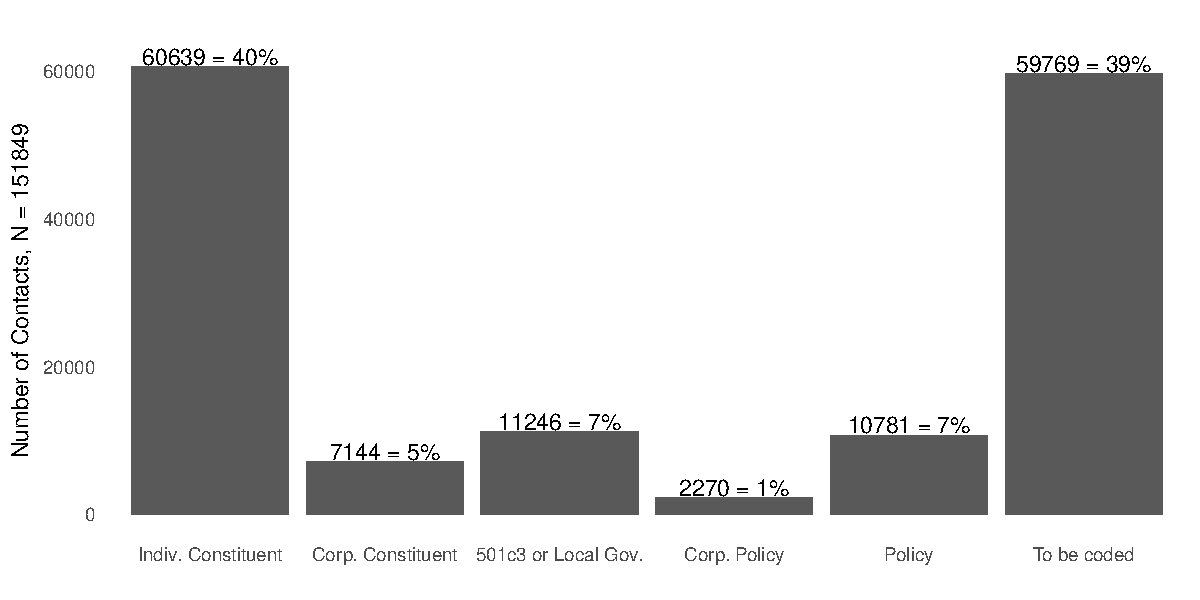
\includegraphics{data_by_type.pdf}}
\end{figure}


\subsubsection{Unequally distributed advocacy}

The number of constituency service requests that legislators write is distributed highly unequally both across and within the House and Senate---evidence that this is behavior that some legislators specialize in, while other legislators engage in only sparingly. Indeed, Senate and House Gini coefficients are comparable to income inequality in the US and Mexico---in short, there is considerable across-legislator variation in how elected officials contact agencies. Furthermore, the same legislators who tend to engage in disproportionately more or less constituent service exhibit a parallel pattern in their policy work. We consider some potential explanations for this variation, before highlighting the role of a legislator's power in Washington.  

% mean per year
% note: I considered changing this to a histogram, but upon reflection, it seems that mean per member per year is a more interesting axis than number per percentile (as a histogram with bin = 100 would show). As a pattern, they look the same. However, I would be interested to hear any counterarguments. 

\begin{figure}
\centering
\caption{Considerable Across Legislator Variation in Who Contacts Agencies}

\includegraphics[width = \textwidth]{percentiles-1}
\end{figure}

\begin{figure}
\centering
\caption{Senators from larger states do more constituent service.}

\includegraphics[width = \textwidth]{population-1}
\end{figure}

\paragraph{Population} An obvious initial explanation for the differences in the rates legislators contact on behalf of their constituents is the population of a district.  After all, legislators are most likely to contact agencies on behalf of their constituents if they receive some request to make that contact.  Of course, House districts have similar populations, so differences in the number of constituents cannot explain the variation in their proclivity to contact the bureaucracy.  The Senate, however, shows strong evidence that the number of constituents influences their level of contact.  In fact, in the Senate, an additional million constituents is associated with an additional 0.15 contacts per agency per year.\footnote{While such numbers may seem small, they are substantive large when considering our units of analysis are mostly sub-departmental agencies or components, of which we identified 234. Even by a conservative estimate, one additional contact per agency may translate to an additional 100 contacts per year government-wide. Thus, we estimate that 0.15 additional contacts per agency indicate roughly 15-30 additional contacts per year.} There are two complementary explanations for this difference. First, it could be that senators from more populous states simply receive more requests for constituency service.  Second, it could be that legislators from larger states are able to make use of their larger staff.  Preliminary, our evidence suggests that demand is a significant driver of unequally distributed advocacy. For every additional million constituents, senators initiate an additional 0.09 contacts per year on behalf of constituents, while only policy contacts only increase by 0.005 per year.  

 This reflects an important input to the number of letters a legislator can produce.  Legislators can initiate letters on their own to advocate for policy, but they are only able to produce letters for constituency service when constituents request their representative's help.  Legislators can solicit their constituents to try and increase the supply of letters, but the total population in the state constrains them.   

%\begin{figure}
%\caption{Population Matters More and Republicans Write More Letters Than Democrats }\label{f:fig_pop}
%
\includegraphics[width = \textwidth]{party_mean_by_month-1}
%\end{figure}

%\begin{figure}
%\caption{New test}
%
\includegraphics[width = \textwidth]{means_by_type-1}
%\end{figure}

% density 

% density by type

\paragraph{Gender} While there is a robust literature on women's overperformance in Congress, there appear to be no systematic differences between the rates men and women contact agencies on behalf of their constituents overall.  Once we take into account idiosyncrasies from agencies and Congressional terms, women write 0.09 fewer letters per agency than their male colleagues, but this difference is not substantively nor statistically significant.  Women also write fewer constituency service requests and fewer requests to revise policy, but again those differences not statistically significant.  However, more nuanced studies have found that female legislators write more on behalf of women \citet{LowandeRitchieLauterbach2018}. 



\section{What Causes Legislators to Write Letters and What Effect Do They Have?}

Our comprehensive data set and panel research designs enable us to address questions about what causes legislators to contact agencies more often on behalf of their constituents and what effects those constituent contacts have on government decision making.  Here, we briefly describe how we can use our data set to understand who provides representation and the consequences of this work.  




\section{Evidence that Power Affects a Legislator's Tendency to Write Letters}

%While the average contacts per member are roughly the same for both parties regardless of majority status in the House, Senate Republicans average more contacts per year while in the minority, while Senate Democrats are the reverse. Contacts rise and fall with legislative sessions, but are not noticeably linked to the electoral calendar. In almost every month from 2007 to 2017, Senate Democrats averaged more letters than Republicans---almost twice as many on average, while they were in the majority. 

%\todo{members by when they are up for re-election}

As a proof of concept, we show how we can examine how a legislator's power affects their propensity to contact federal agencies.  A legislator's characteristics and the characteristics of their district are related to the rate of contacting federal agencies.  So too is a legislator's position in the institution.  Consider the results presented in Table \ref{t:Cross}.  This shows that legislators who are in a position of power tend to initiate more contacts with the bureaucracy.  For example, members of prestige committees wrote an additional 1.1 letters per agency---0.68 of which were for constituent service and 0.04 were on policy concerns, compared to members of Congress not on prestigious committees.  Similarly, senators and representatives who are committee chairs write more letters---an additional 1.5 per agency, while chairs of prestige committees wrote an additional 1.8 letters per agency.  (Please note, that because not all letters have been coded, the basic arithmetic that we might expect to work will fail, as the total number of letters (the left-hand column in the table) includes letters that are yet to be coded.)

Of course, we should exercise caution when interpreting these results, because legislators who are more productive letter writers are also more likely to be selected for prestigious committees or to be committee chairs.  For example, in the period before they become chairs legislators who will eventually become committee chairs write an additional 1.1 letters per agency, a statistically significant increase over their colleagues who will not become chairs.  

The cross-sectional comparisons, then, conflates the power a legislator is able to utilize after becoming a chair with the selection of individual legislators.  We see a similar, though smaller increase across legislators who are both in the majority and in the president's party.  Members of the president's party, when they are in the majority, write about an additional 0.6 letters per agency, a statistically significant difference.  But when only in the majority or when they only are in the same party as the president but in the minority, they write fewer letters.  This can be attributed, in part, to the fact that Senate Democrats lobby the bureaucracy more than Republicans regardless of majority status and happened to be in the majority for most of 2009-2016 when their partisan was president and lost the majority at the same time Democrats lost the presidency. 

\begin{table}[hbt!]
\centering
\caption{Cross Sectional Differences in Letter Writing}\label{t:Cross}
\begin{tabular}  {l|ccc}
                &  Overall & Constituent & Policy    \\
Prestige Comm. &  1.10    &  0.68            &  0.04         \\
                & (0.06)  &   (0.05)          &  (0.01)         \\
\hline \hline             
       Chair    & 1.51        & 0.59             &  0.23         \\
                &  (0.09)     & (0.08)            &  (0.02)         \\
\hline \hline                
Prestige Chair    &  1.80        &  1.05           &   0.12        \\
                &   (0.16)       &  (0.14)           &  (0.03)         \\
\hline \hline                 
    Majority    &    -2.15      &  -1.36           & -0.14          \\
                &     (0.12)     &  (0.10)           & (0.02)          \\                
President's Party&   -2.10       &   -1.33          & -0.12          \\    
                &     (0.12)     &    (0.10)         &  (0.02)         \\
Majority x President's Party & 4.80         & 2.91             &  0.29         \\    
                              & (0.19)      & (0.16)             &  (0.4)         \\
\hline 
Congress Fixed Effects           &  \checkmark   &     \checkmark        &    \checkmark     \\
Agency Fixed Effects           &  \checkmark   &      \checkmark    & \checkmark    \\    
\hline 
\hline        
\end{tabular}
\end{table}



%\begin{figure}
%\caption{Test 4}
%
\includegraphics[width = \textwidth]{party_distance_above_mean-1}
%\end{figure}

While we are unable to use overtime variation to assess the effect of district characteristics or the immutable legislator traits, we can use the changing composition of committees and committee chairpersons to better isolate the effect of additional power.  To do this, we investigate similar differences as Table \ref{t:Cross}, but now use a difference-in-differences design \citep{BerryFowler2016}.  The difference-in-differences design compares changes in legislators who either acquire or lose some power---like the chair of a committee--with those legislators whose position remains unchanged.  This trend enables us to isolate any time-invariant characteristics of legislators, such as their ability to more efficiently use their office resources to perform constituency service. 

Table \ref{t:did} shows the results of four distinct DiD designs: the effect of being on a prestige committee, holding a chair, the chair of a prestige committee, and a design to assess the effect of institutional power that comes from being in the majority or from the same party as the president.  This design reveals that as legislators acquire power, they write more letters to agencies.  For example, becoming a chair of a committee causes a very large substantive increase of 0.59 letters per agency from the legislator.  We see a similar increase from becoming a chair of a prestige committee.  Our tentative coding of the letters shows that there are increases in both requests for individual constituent service and for policy.  Further, we see a similar slight increase that comes when legislators are both in the majority and from the same party as the president, indicating that the positive effect of majority control with a copartisan president is not merely driven by the position of Senate Democrats in our time period. 



\begin{table}[hbt!]
\centering
\caption{Difference-in-Differences in Letter Writing}\label{t:did}
\begin{tabular} {l|ccc} 
                &  Overall & Constituent & Policy    \\
Prestige Comm. &  0.16    &  0.05            &  -0.04         \\
                & (0.15)  &   (0.14)          &  (0.03)         \\
\hline \hline             
       Chair    & 0.59        & 0.07            &  0.16         \\
                &  (0.14)     & (0.12)            &  (0.03)         \\
\hline \hline                
Prestige Chair    &  0.58        &  0.31           &    0.07      \\
                &   (0.25)       &  (0.23)           &  (0.05)         \\
\hline \hline                 
    Majority    &    -0.45      &  -0.38           & -0.14          \\
                &     (0.16)     &  (0.14)           & (0.02)          \\                
President's Party&   -0.30       &   -0.35          & -0.12          \\    
                &     (0.15)     &    (0.13)         &  (0.02)         \\
Majority x President's Party & 1.02         & 0.88            &  0.02        \\    
                              & (0.25)      & (0.22)             &  (0.05)         \\
\hline 
Congress Fixed Effects           &  \checkmark        &     \checkmark       &     \checkmark     \\
Agency Fixed Effects           &  \checkmark           &       \checkmark    & \checkmark    \\    
Legislator Fixed Effects         & \checkmark             &   \checkmark         & \checkmark \\
\hline \hline         
\end{tabular}
\end{table}

There are, of course, a number of mechanisms that could explain these results. First, constituents might rationally reach out to elected officials more often when those officials hold additional power. Second, it could be that as elected officials acquire more power they draw on the resources of their office to shore up their electoral base.  Third, it could be a combination of the two, where additional power raises a legislator's prestige and makes it more likely that constituents are aware of who their elected official is and that their representative can be an effective advocate on their behalf when dealing with an agency. 

As a preliminary test of these different explanations Table \ref{t:over} compares the rate that chairs of committee with oversight power over an agency write to that agency to the rate other members of the same committee write to the same agency. In the cross-sectional comparison, it is clear that chairs, compared to the other members of their committee, write more often to the agencies over which they have statutory oversight.  Further, a DiD design shows that this effect is very large--an additional 5 letters per agency the chair has discretion over, relative to the other committee members.  And, our preliminary coding of the letters shows that this increase is largely related to constituent service, suggesting that committee chairs use their formal power for more than policy oversight. 


\begin{table}[hbt!]
\centering
\caption{Chairs of Committees with Oversight Power Allocate More Attention to Individual Requests Than Other Committee Members }\label{t:over}
\begin{tabular}{l|ccc||ccc}
                  &Overall & Constituent             & Policy & Overall & Constituent & Policy \\
Oversight Chair & 2.62          &        1.70        & 0.40     &     5.05   & 3.78         & 0.21        \\
                & (0.56)          &        (0.54)        & (0.10) &     (1.04) & (0.95)         & (0.17)        \\
\hline
Congress FE        &     \checkmark      &    \checkmark            & \checkmark         &     \checkmark        &         \checkmark      &     \checkmark    \\
Agency FE         &     \checkmark      &\checkmark                & \checkmark         &     \checkmark        & \checkmark          & \checkmark        \\
Legislator FE   &                     &                        &                     & \checkmark          &     \checkmark          &     \checkmark    \\
\hline \hline 
\end{tabular}
\end{table}

That is, when legislators gain power over a part of the federal bureaucracy, they increase their interaction with those agencies by advocating for their constituents.  This evidence suggests that elected officials use powerful offices to do more than impose their policy preferences. It shows that chairs use their office to more often advocate for their constituents in exactly the venues where they have the greatest leverage to do so. 

\subsection{The Effect of Constituent Requests on Government Decision Making }
Our data and design also enable us to assess how constituent service requests affect how bureaucrats allocate funds.  As we mention above we adopt two broad strategies for assessing how constituent service requests affect how money is allocated by the federal government. 

We plan to leverage changes in the institutional rules that shifted more freedom to bureaucratic agencies to allocate funds.  Specifically, in the past decade, Congress has instituted bans on lawmakers ``earmarking" funds in appropriation bills. This practice enabled lawmakers to designate money appropriated to federal agencies to be spent on specific projects, usually in the lawmaker's state or district.  The ban on earmarking enabled agencies to make this decision.  But of course, we might expect that agencies feel pressure from particular lawmakers to allocate funds.  If this is true, then similar earmarking decisions could be made, but with substantially less transparency than before.  To assess whether this occurs, we will compare the types of service requests lawmakers made before and after the imposition of the earmark ban.  If we see a marked increase in service requests to agencies that previously had a large share of earmarked funds, then we have circumstantial evidence that lawmakers are attempting to influence the allocation process. 

We can build a more direct case by examining the relationship between lawmakers writing letters in support of grants and the rate those grants are actually allocated.  To do this, we will link our database on letters of support from lawmakers to agencies with actual appropriation decisions from the agency.  Of course, the relationship may not be causal.  But we plan to use the timing of the letter and comparisons within agencies and within legislators to ensure that we are not merely detecting differences across districts or an individual legislator's own propensity to ``time" their letters correctly. 


\section{Conclusion}





More importantly, looking across many agencies reveals that powerful legislators like committee chairs use their power to advocate for their constituents across the vast federal bureaucracy. This aligns with the findings of \citet{RitchieYou2018} that the Department of Labor was contacted and influenced by a wide array of members, with no special treatment for those with formal oversight powers. But institutional power matters beyond formal oversight. While de jure, agency-specific oversight may be weaker than commonly assumed, institutional positions appear to increase de facto oversight over much broader swaths of government. When institutional power is attained, elected officials do use institutional power to press their policy agendas \emph{and} to advocate for their constituents.

%\citet{Carney1994}

\bibliographystyle{chicago-apsr}

\bibliography{congress2018}

%\newpage
%\listoftodos[Notes]


\end{document}






